% ICASSP 2027 submission — CROA (official spconf template)
% Compiled against PaperFormat/spconf.sty + IEEEbib.bst from the ICASSP 2027 paper kit.
\documentclass{article}
\usepackage{spconf,amsmath,amssymb,graphicx,booktabs,balance,indentfirst}
\usepackage[colorlinks=true,linkcolor=blue,citecolor=blue,urlcolor=blue]{hyperref}
\renewcommand{\topfraction}{0.95}
\renewcommand{\textfraction}{0.05}
\setlength{\textfloatsep}{9pt plus 2pt minus 3pt}
\setlength{\dbltextfloatsep}{9pt plus 2pt minus 3pt}
\setlength{\abovecaptionskip}{4pt}
\setlength{\belowcaptionskip}{2pt}
\renewcommand{\textfraction}{0.05}

\newcommand{\ours}{\textsc{CROA}}

\title{CROA: CROSS-REPRESENTATION OPTIMAL ALIGNMENT FOR\\ FINE-GRAINED TARGETED TRANSFER ATTACKS ON MLLMS}

\name{Junxi Chen$^{1\dagger}$, Max He$^{2\dagger}$, Jiahao Zhang$^1$, Xiaoli Zhao$^1$, Jinyi Pang$^1$, Zuyi Li$^3$, and Yilin Wu$^{4\ast}$}
\address{$^1$South China University of Technology \quad $^2$University of British Columbia \\
$^3$Shaanxi Normal University \quad $^4$Guangdong University of Education\\}

\begin{document}
\ninept

\maketitle


\let\thefootnote\relax
\footnotetext{$^{\dagger}$Equal contribution. \quad $^{\ast}$Corresponding author.}

\begin{abstract}
Multimodal large language models (MLLMs) are exposed to targeted
transfer attacks that steer a black-box victim toward attacker-chosen
semantics using perturbations optimized on surrogate encoders. For
\emph{fine-grained} targeting, existing attacks predominantly draw
their surrogates from the image--text contrastive paradigm, which focuses
on high-level semantic categories but may under-constrain fine-grained spatial
details. We propose \ours{} (Cross-Representation Optimal Alignment),
integrating contrastive and self-supervised representations where the
two paradigms provide complementary local visual information. CROA couples
a multi-architecture CLIP ensemble with DINOv2 by establishing clustered
local optimal transport across patch tokens in both feature spaces alongside
global feature alignment. It further incorporates source repulsion and
multi-crop momentum optimization under a unified configuration.
Extensive experiments across six commercial and open-source MLLM victims
show that \ours{} achieves the highest mean ASR among the evaluated methods
under our benchmark settings, attaining 51.0\% on commercial frontier models
and 92.0\% on open-source models, outperforming both single- and
multi-paradigm baselines. Code is available at \url{https://github.com/chenwudao/CROA}.
\end{abstract}

\begin{keywords}
Adversarial attack, targeted transfer attack, multimodal language model,
optimal transport, fine-grained targeting
\end{keywords}

\begin{figure}[t]
\centering
\makebox[\columnwidth][c]{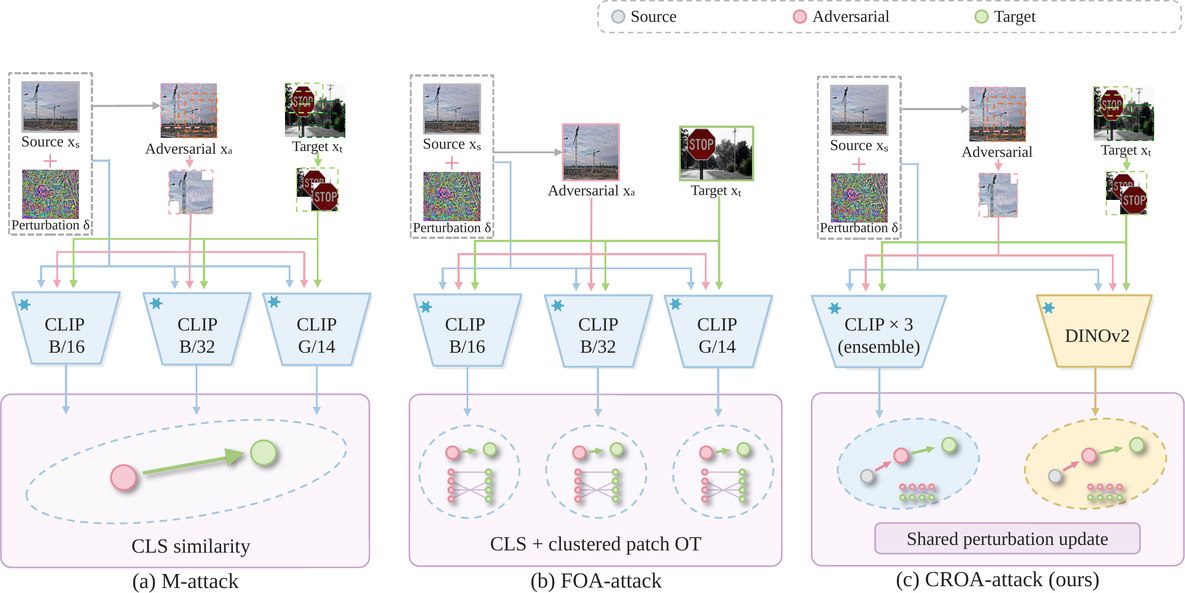
\includegraphics[width=1.02\columnwidth]{assets/ppt_fig1_motivation.png}}
\par\vspace{4pt}
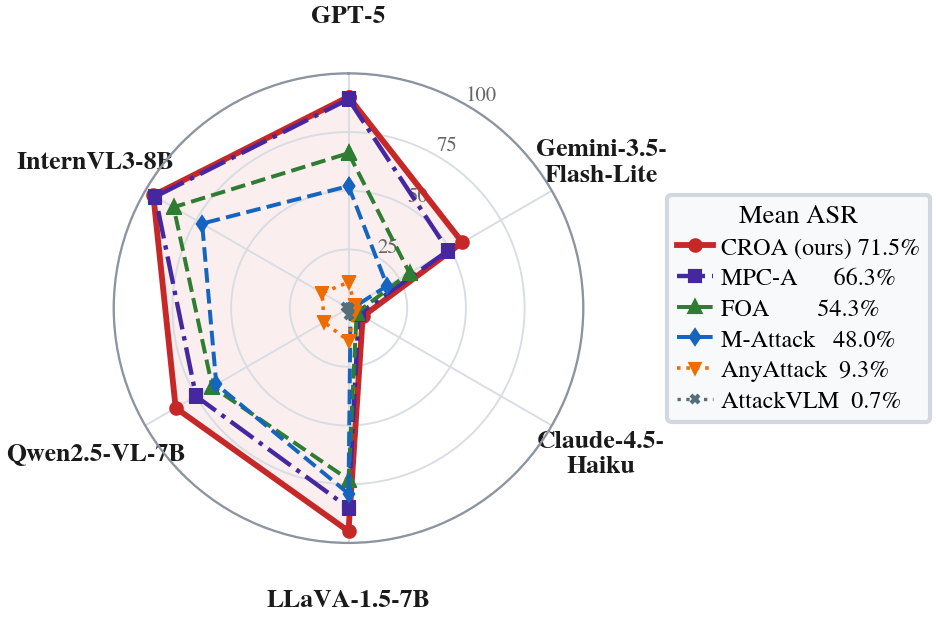
\includegraphics[width=0.86\columnwidth]{assets/fig1_radar_enlarged.png}
\vspace{-4pt}
\caption{From single-paradigm to cross-representation alignment.
Top: (a) M-Attack, (b) FOA, and (c) CROA architectures. Bottom:
Targeted ASR (\%) across six commercial and open-source victims,
with aggregate 6-victim mean in the legend.}
\label{fig:motivation}
\end{figure}

\begin{figure*}[t]
\centering
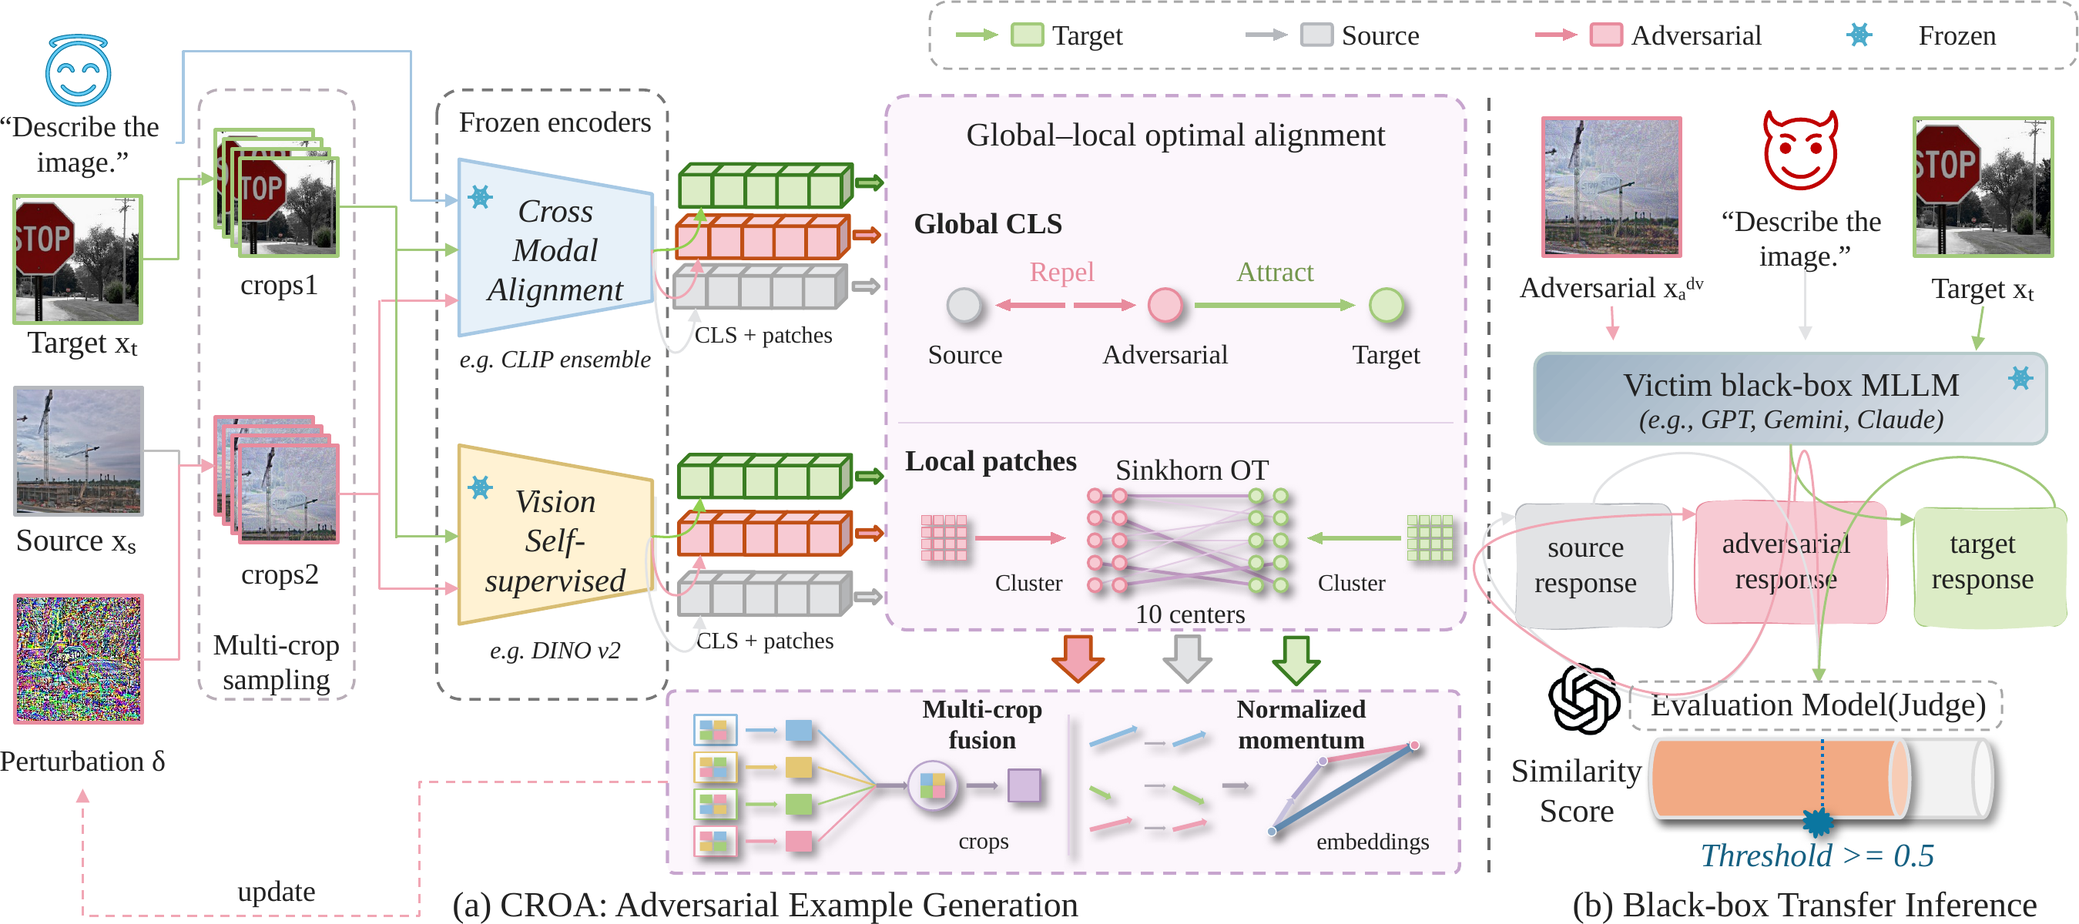
\includegraphics[width=0.88\textwidth]{assets/ppt_fig2_method.png}
\caption{CROA overview. Frozen CLIP and DINOv2 encoders provide global
and local target-alignment objectives. Global source repulsion complements
target attraction; clustered patch OT supplies local matching. Four-view
averaging and normalized momentum update a shared perturbation. Victim
captions and target references are compared only at evaluation time.}
\label{fig:method}
\end{figure*}

\section{Introduction}
Multimodal large language models (MLLMs)~\cite{flamingo,blip2} have
achieved remarkable progress in visual understanding and natural
language generation. As MLLMs are increasingly deployed in
real-world applications, their vulnerability to adversarial examples
has become a pressing security concern~\cite{attackvlm}. Among
various attack surfaces, \emph{targeted transfer attacks} are
particularly practical: perturbations are optimized on locally
available surrogate encoders and transferred to black-box victims
with zero queries, steering the victim's caption toward an
attacker-chosen target image~\cite{mattack,foa}.

Along this line, AttackVLM~\cite{attackvlm} aligns projected CLIP
features via ensemble cosine similarity. ITA~\cite{ita} investigates
imperceptible transfer attacks under perturbation constraints. M-Attack~\cite{mattack}
introduces random-crop augmentation on CLS embeddings, showing that
input diversity enhances transferability. FOA-Attack~\cite{foa} couples
global CLS cosine alignment with local optimal transport (OT) on clustered
patch tokens to match feature distributions within contrastive feature space.
Despite this algorithmic progression, these methods remain confined
to the image--text contrastive paradigm. Contrastive pretraining optimizes
cross-modal alignment, which captures high-level semantics effectively but
may provide limited localized visual structure. In contrast, self-supervised
representations provide rich, complementary local patch features.

To leverage multiple paradigms, MPCAttack~\cite{mpcattack} combines CLIP,
DINOv2, and an auxiliary MLLM surrogate with a source-repulsion term.
However, it relies on \emph{coarse global pooling}, concatenating 1D global
vectors (such as DINOv2 CLS tokens) into a joint similarity objective while
requiring target text prompts and white-box MLLM queries during optimization.
By discarding dense patch tokens in the self-supervised branch, it cannot
exploit the complementary spatial and structural details preserved in DINOv2 patch fields.
Under the tight $L_\infty$ budget, residual source features can also persist,
leading to ``double exposure'' captions that conflate source and target concepts.

To address these limitations, we propose Cross-Representation
Optimal Alignment (\ours{}). Unlike prior works that perform patch-level
optimal transport only within contrastive models~\cite{foa} or collapse
self-supervised representations to global pooled vectors~\cite{mpcattack},
CROA establishes fine-grained local optimal transport across patch tokens
in \emph{both} CLIP and DINOv2 feature spaces. In a vision-only
setting without target text or MLLM surrogates, CROA couples
global alignment with clustered local OT, incorporates cross-representation
source repulsion, and stabilizes updates with multi-crop normalized momentum.

Our main contributions are summarized as follows:
\begin{itemize}
\item We propose a vision-only cross-representation attack framework
that performs local optimal transport across both contrastive and
self-supervised patch spaces alongside global alignment and source repulsion,
generating transferable perturbations without target text or MLLM surrogates.
\item We evaluate CROA across three commercial frontier MLLMs
(GPT-5, Gemini-3.5-FL, Claude-4.5-H) and three open-source MLLMs
(LLaVA-1.5, Qwen2.5-VL, InternVL3), achieving top mean ASR on both
commercial (51.0\%) and open-source models (92.0\%, exceeding
MPC-A by 7.0 points), with an overall 71.5\% mean across all six victims.
\item We provide component ablations isolating representation paradigm,
local OT, and source repulsion across all six architectures,
demonstrating their contributions to aggregate attack success.
\end{itemize}

\section{Methodology}
\subsection{Preliminaries}
Let $\mathcal{V}$ denote a black-box victim MLLM that generates caption
$y = \mathcal{V}(x, p)$ given an input image $x$ and a fixed captioning
prompt $p$ (``Describe this image in one concise sentence, no longer
than 20 words.''). Given a source image $x_s$ and an attacker-chosen
target image $x_t$ whose target caption is $y_t = \mathcal{V}(x_t, p)$,
the adversary seeks an adversarial perturbation $\delta$ bounded by
$\|\delta\|_\infty \le \varepsilon$ ($\varepsilon = 16/255$) to steer
the victim's caption toward the target concept:
\begin{equation}\label{eq:blackbox_goal}
\max_{\|\delta\|_\infty \le \varepsilon} \mathcal{S}\left(\mathcal{V}(\operatorname{clip}_{[0,1]}(x_s + \delta), p), \, y_t\right),
\end{equation}
where $\mathcal{S}(\cdot, \cdot)$ measures semantic similarity via an
LLM judge. Because $\mathcal{V}$ is query-free and gradient-inaccessible,
direct optimization of Eq.~\eqref{eq:blackbox_goal} is impossible.
Instead, the adversary optimizes an adversarial surrogate objective
$\mathcal{L}_{\mathrm{CROA}}$ over a local surrogate ensemble~$\mathcal{F}$:
\begin{equation}\label{eq:surrogate_opt}
\delta^* = \arg\max_{\|\delta\|_\infty \le \varepsilon} \mathcal{L}_{\mathrm{CROA}}(x_s + \delta, \, x_t, \, x_s; \, \mathcal{F}),
\end{equation}
and directly transfers $x = \operatorname{clip}_{[0,1]}(x_s + \delta^*)$
to $\mathcal{V}$ with zero victim queries. Fig.~\ref{fig:method}
illustrates the overall framework.

\subsection{Cross-paradigm surrogate fusion}
\begin{table}[t]
\centering
\caption{Surrogate interfaces. DINOv2-B/14 exposes the same
CLS/patch-token interface as the contrastive extractors.}
\label{tab:interface}
\small
\setlength{\tabcolsep}{3pt}
\begin{tabular}{lccc}
\toprule
Extractor & Paradigm & CLS dim & Patches \\
\midrule
CLIP-B/16 & contrastive & 768 & $196{\times}768$ \\
CLIP-B/32 & contrastive & 768 & $49{\times}768$ \\
LAION-G/14 & contrastive & 1408 & $256{\times}1408$ \\
DINOv2-B/14 & self-sup. & 768 & $256{\times}768$ \\
\bottomrule
\end{tabular}
\end{table}

% AUDITED_MAIN_TABLE
\begin{table*}[t]
\centering
\caption{Targeted ASR (\%) on three commercial victims. Bold marks column maxima.}
\label{tab:main}
\small
\setlength{\tabcolsep}{8pt}
\begin{tabular}{lrrrrrrrr}
\toprule
& \multicolumn{2}{c}{GPT-5} & \multicolumn{2}{c}{Gemini-3.5-FL} & \multicolumn{2}{c}{Claude-4.5-H} & \multicolumn{2}{c}{Mean} \\
Method & ASR & KMR & ASR & KMR & ASR & KMR & ASR & KMR \\
\midrule
AttackVLM~\cite{attackvlm} & 0.0 & 6.0 & 0.0 & 4.2 & 0.0 & 4.1 & 0.0 & 4.7 \\
AnyAttack~\cite{anyattack} & 11.0 & 14.8 & 3.0 & 9.1 & 3.0 & \textbf{10.5} & 5.7 & 11.5 \\
M-Attack~\cite{mattack} & 52.0 & 49.1 & 19.0 & 28.6 & 1.0 & 7.4 & 24.0 & 28.4 \\
FOA~\cite{foa} & 66.0 & 51.8 & 30.0 & 32.2 & 4.0 & 9.8 & 33.3 & 31.3 \\
MPC-A~\cite{mpcattack} & 89.0 & 65.0 & 49.0 & 43.2 & 5.0 & 10.2 & 47.7 & 39.5 \\
\ours{} & \textbf{90.0} & \textbf{65.1} & \textbf{56.0} & \textbf{49.3} & \textbf{7.0} & 9.5 & \textbf{51.0} & \textbf{41.3} \\
\bottomrule
\end{tabular}
\end{table*}
% END_AUDITED_MAIN_TABLE
Fig.~\ref{fig:method}(a) illustrates the surrogate pipeline. The contrastive branch $\mathcal C$ comprises CLIP-B/16, CLIP-B/32,
and LAION CLIP-G/14~\cite{clip,laion}; the self-supervised branch $d$
is DINOv2-B/14~\cite{dinov2}. For every encoder $k$, we extract the
final-layer CLS token $f^{\mathrm{cls}}_k(x)$ and patch tokens
$\{f^{\mathrm{tok}}_{k,\ell}(x)\}_{\ell=1}^{N_k}$, $\ell_2$-normalizing each:
\begin{equation}
c_k(x)=\frac{f^{\mathrm{cls}}_k(x)}{\|f^{\mathrm{cls}}_k(x)\|_2},\quad
p_{k,\ell}(x)=\frac{f^{\mathrm{tok}}_{k,\ell}(x)}{\|f^{\mathrm{tok}}_{k,\ell}(x)\|_2}.
\end{equation}
While CLIP aligns images with natural language to provide high-level
semantic guidance, DINOv2 provides complementary local visual features
capturing spatial layout and object structure. Crucially, unlike
MPCAttack~\cite{mpcattack}, which collapses DINOv2 into a single CLS
token and relies on target text guidance alongside an MLLM surrogate,
CROA preserves full patch token fields in both paradigms and performs
fine-grained local optimal transport within their native metric spaces
in a purely vision-to-vision setting.

\subsection{Source-aware global--local OT alignment}
\textbf{Global attraction and repulsion.} As shown in Fig.~\ref{fig:method}(b),
optimizing solely toward the target without penalizing source similarity
can leave residual source patterns under a tight $L_\infty$ budget,
inducing double exposure. We thus incorporate global attraction and source repulsion
in each encoder space:
\begin{equation}\label{eq:global_rep}
G_k(x)=c_k(x)^\top c_k(x_t)-\beta\, c_k(x)^\top c_k(x_s),
\end{equation}
where $\beta=0.5$ is shared across both branches; the second term
expels residual source features from both contrastive ($\mathcal{C}$)
and self-supervised ($d$) representation spaces.
Source references $\{c_k(x_s)\}$ are precomputed once from the clean image.

\textbf{Local clustered transport.} Following FOA's formulation~\cite{foa},
we match patch token distributions via optimal transport. Patch tokens
of each crop are assigned to $K_c=10$ clusters by iterative maximum-dot-product
assignment; each centroid $a_i=|S_i|^{-1}\sum_{p\in S_i}p$ is a token mean,
with $B=\{b_j\}_{j=1}^{K_c}$ obtained analogously for the target. On the
similarity matrix $S_{ij}=a_i^\top b_j$, we run entropic Sinkhorn
iterations~\cite{sinkhorn,cuturi} on the Gibbs kernel
$K_{ij}=\exp[(S_{ij}-1)/0.1]$ under uniform marginals:
\begin{equation}\label{eq:sinkhorn}
u\leftarrow \frac{\mathbf 1/K_c}{K v},\qquad
v\leftarrow \frac{\mathbf 1/K_c}{K^\top u},
\end{equation}
for at most 100 iterations or until convergence ($<10^{-2}$). The resulting
plan $\mathbf P^*=\operatorname{diag}(u)K\operatorname{diag}(v)$ is detached
from the graph, and the local objective transports feature content through:
\begin{equation}\label{eq:local_ot}
T_k(x)=\sum_{i=1}^{K_c}\sum_{j=1}^{K_c}\mathbf P^*_{ij}\,a_i^\top b_j.
\end{equation}
Stop-gradients through $\mathbf P^*$ and discrete assignments allow
gradients to flow directly through the centroid means.

\textbf{Cross-representation objective.} With
$L_k=G_k+\lambda_kT_k$, where $\lambda_C=0.2$ for CLIP and
$\lambda_D=0.4$ for DINOv2, the fused objective balances both
paradigms:
\begin{equation}\label{eq:croa_loss}
L_{\mathrm{CROA}}=\frac{0.5}{|\mathcal C|}\sum_{k\in\mathcal C}L_k+0.5\,L_d.
\end{equation}
The three CLIP encoders share half the objective and DINOv2 receives
the other half, preventing encoder count from dominating either
paradigm. Furthermore, DINOv2 employs a stronger local weight
($\lambda_D=0.4$ vs.\ $\lambda_C=0.2$) because self-supervised tokens
provide complementary local visual features that capture localized structure,
tolerating richer local transport without corrupting global semantics.

\subsection{Multi-crop momentum optimization}
At each step, we sample $M=4$ independent source and target views with
crop area fractions in $[0.35,1.0]$ to capture multi-scale contexts.
Unlike unnormalized momentum in prior attacks~\cite{mpcattack}, we average
multi-crop losses and apply mean-absolute gradient normalization~\cite{mifgsm}:
\begin{align}
L&=M^{-1}\sum_{m=1}^{M}L_{\mathrm{CROA}}^{(m)},\label{eq:avg}\\
m_{t+1}&=\mu\,m_t+\frac{\nabla_\delta L}{\operatorname{mean}|\nabla_\delta L|+10^{-8}},\notag\\
\delta_{t+1}&=\Pi_{\|\delta\|_\infty\le\varepsilon}
\left(\delta_t+\alpha\,\operatorname{sign}(m_{t+1})\right),\notag
\end{align}
with $\mu=0.9$, $\alpha=1/255$, $\delta_0=m_0=0$, and $T=300$ steps.
Mean normalization decouples step magnitude from loss-scale differences
across paradigms, stabilizing gradient stochasticity from multi-crop
sampling and patch clustering. All hyperparameters are shared across
victims without any per-victim tuning.

\section{Experiments}
\subsection{Experimental settings}
\textbf{Baselines.} We compare \ours{} with representative transferable adversarial attack methods on MLLMs, including AttackVLM~\cite{attackvlm}, AnyAttack~\cite{anyattack}, M-Attack~\cite{mattack}, FOA~\cite{foa}, and MPC-A~\cite{mpcattack}. Baselines are reproduced following their open-source implementations, adapting text inputs where required (such as target descriptions for MPC-A), under unified perturbation budgets, test samples, and evaluation pipelines.

\textbf{Datasets and victims.} Following the standard benchmark protocols of M-Attack~\cite{mattack} and FOA~\cite{foa}, we adopt the 100 source--target image pairs constructed from the NIPS 2017 Adversarial Attacks and Defenses Competition dataset along with their fine-grained target keyword annotations to ensure a fair and consistent comparison. Evaluated victims encompass both representative closed-source commercial models (GPT-5~\cite{gpt5}, Gemini-3.5-Flash-Lite~\cite{gemini}, and Claude-4.5-Haiku~\cite{claude}) and popular open-source MLLMs (LLaVA-1.5-7B~\cite{llava}, Qwen2.5-VL-7B~\cite{qwenvl}, and InternVL3-8B~\cite{internvl}).

\textbf{Attack configurations.} Following standard practice~\cite{foa,mpcattack}, all iterative attacks run for $T=300$ steps under an $L_\infty$ perturbation budget of $\varepsilon=16/255$ with step size $\alpha=1/255$. For \ours{}, hyperparameters are set to $\beta=0.5$, $\lambda_C=0.2$, $\lambda_D=0.4$, $w_C=w_D=0.5$, $M=4$ crops in $[0.35,1.0]$, and momentum $\mu=0.9$, kept strictly frozen across all victims. All perturbation generation runs on a single NVIDIA RTX~6000~Ada (48\,GB) GPU.

\textbf{Evaluation metrics.} Following the evaluation protocol of FOA~\cite{foa}, we adopt the LLM-as-a-judge framework using GPT-4o-mini~\cite{gpt4}. We evaluate two primary metrics: (1) \textbf{Targeted ASR}: following FOA's prompting format inspired by GPTScore~\cite{gptscore}, GPT-4o-mini directly scores the semantic similarity between the victim caption and target description; an attack succeeds if the score is $\ge 0.5$. (2) \textbf{Keyword Match Rate (KMR)}: GPT-4o-mini evaluates the recall of target-specific keywords within the victim caption, measuring fine-grained semantic transfer fidelity.

\subsection{Main results}
Table~\ref{tab:main} reports targeted attack results on three commercial victims. \ours{} attains the highest aggregate ASR (51.0\%) and KMR (41.3\%) among evaluated baselines under our benchmark settings, outperforming MPC-A (47.7\% ASR, 39.5\% KMR) and FOA (33.3\% ASR, 31.3\% KMR). This demonstrates that jointly aligning contrastive semantics and dense self-supervised geometry substantially enhances cross-model transferability in a vision-only setting. On GPT-5 and Gemini-3.5-FL, \ours{} achieves 90.0\% and 56.0\% ASR, improving over FOA by 24.0 and 26.0 percentage points, respectively. While Claude-4.5-H remains challenging across all evaluated attacks, \ours{} still achieves the highest ASR of 7.0\%. Furthermore, \ours{} demonstrates superior semantic fidelity, reaching 65.1\% KMR on GPT-5 and 49.3\% on Gemini.

% AUDITED_OPEN_TABLE
\begin{table}[t]
\centering
\caption{Open-source ASR (\%). A three-model mean is reported across all evaluated architectures (100 pairs each).}
\label{tab:opensource}
\small
\setlength{\tabcolsep}{3.5pt}
\begin{tabular}{lrrrr}
\toprule
Method & LLaVA & Qwen2.5 & InternVL3 & Mean \\
\midrule
AttackVLM~\cite{attackvlm} & 3.0 & 0.0 & 1.0 & 1.3 \\
AnyAttack~\cite{anyattack} & 14.0 & 12.0 & 13.0 & 13.0 \\
M-Attack~\cite{mattack} & 79.0 & 65.0 & 72.0 & 72.0 \\
FOA~\cite{foa} & 73.0 & 67.0 & 86.0 & 75.3 \\
MPC-A~\cite{mpcattack} & 85.0 & 75.0 & 95.0 & 85.0 \\
\ours{} & \textbf{95.0} & \textbf{85.0} & \textbf{96.0} & \textbf{92.0} \\
\bottomrule
\end{tabular}
\end{table}
% END_AUDITED_OPEN_TABLE

The open-source panel (Table~\ref{tab:opensource}) gives CROA a
92.0\% mean ASR, versus 85.0\% for MPC-A and 75.3\% for FOA, achieving
95.0\% on LLaVA, 85.0\% on Qwen2.5-VL, and 96.0\% on InternVL3.
A paired exact McNemar test confirms the significance of CROA's gain
over FOA on LLaVA ($p < 0.0001$, 23 wins vs.\ 1 loss; $p=0.021$ vs.\ MPC-A). Across these diverse architectures, the
frozen surrogate ensemble transfers effectively without victim-specific tuning.

\subsection{Ablation study}
% AUDITED_ABLATION_TABLE
\begin{table}[t]
\centering
\caption{Component analysis: ASR (\%) across all six commercial and open-source victims (100 pairs each). Bold marks column maxima.}
\label{tab:ablation}
\small
\resizebox{\columnwidth}{!}{%
\setlength{\tabcolsep}{2.5pt}
\begin{tabular}{lrrrrrrr}
\toprule
Variant & GPT-5 & Gemini & Claude & LLaVA & Qwen & IVL3 & Mean \\
\midrule
FOA (CLIP) & 66 & 30 & 4 & 73 & 67 & 86 & 54.33 \\
CLIP + Multi-scale & 83 & 48 & 5 & 85 & 76 & 92 & 64.83 \\
\midrule
CROA w/o DINOv2 & 89 & 56 & \textbf{9} & 92 & 79 & 88 & 68.83 \\
CROA w/o local OT & 88 & \textbf{60} & 6 & 89 & 81 & 95 & 69.83 \\
CROA w/o repulsion & 85 & 57 & 4 & 91 & 79 & 95 & 68.50 \\
Full \ours{} & \textbf{90} & 56 & 7 & \textbf{95} & \textbf{85} & \textbf{96} & \textbf{71.50} \\
\bottomrule
\end{tabular}%
}
\end{table}
% END_AUDITED_ABLATION_TABLE

\textbf{Representation complementarity.} Table~\ref{tab:ablation}
evaluates each component across all six target architectures.
Compared with the CLIP+Multi-scale baseline, full CROA improves mean ASR by
6.67 points (64.83\% to 71.50\%), reaching consistent gains across victims.
Ablating DINOv2 reduces mean ASR to 68.83\%, with pronounced drops on modern
dense-patch open-source models: InternVL3 falls by 8 points (96\% to 88\%) and
Qwen2.5 falls by 6 points (85\% to 79\%), alongside target-detail KMR
gains from DINOv2 (e.g., GPT-5 KMR: 61.4\% to 65.1\%; LLaVA KMR: 64.0\% to 67.4\%).
While Claude marginally favors CLIP alone (9\% vs.\ 7\%), DINOv2 provides crucial
geometric transferability on vision-centric backbones.

\textbf{Local matching and source awareness.} Removing local OT
reduces mean ASR to 69.83\%, triggering a six-point drop on LLaVA (95\% to 89\%)
and a four-point drop on Qwen2.5 (85\% to 81\%), confirming the value of
patch-level distribution alignment. Removing source repulsion incurs the
heaviest penalties on high-capacity models: GPT-5 drops by 5 points (90\% to 85\%),
Qwen2.5 by 6 points (85\% to 79\%), and LLaVA by 4 points (95\% to 91\%),
reducing mean ASR to 68.50\%. Full CROA achieves the top mean ASR (71.50\%)
and dominates on four of six victims, demonstrating that dual-paradigm alignment,
fine-grained local transport, and active source repulsion collectively contribute
to overall transferability.

\subsection{Qualitative results}
\begin{figure}[t]
\centering
\makebox[\columnwidth][c]{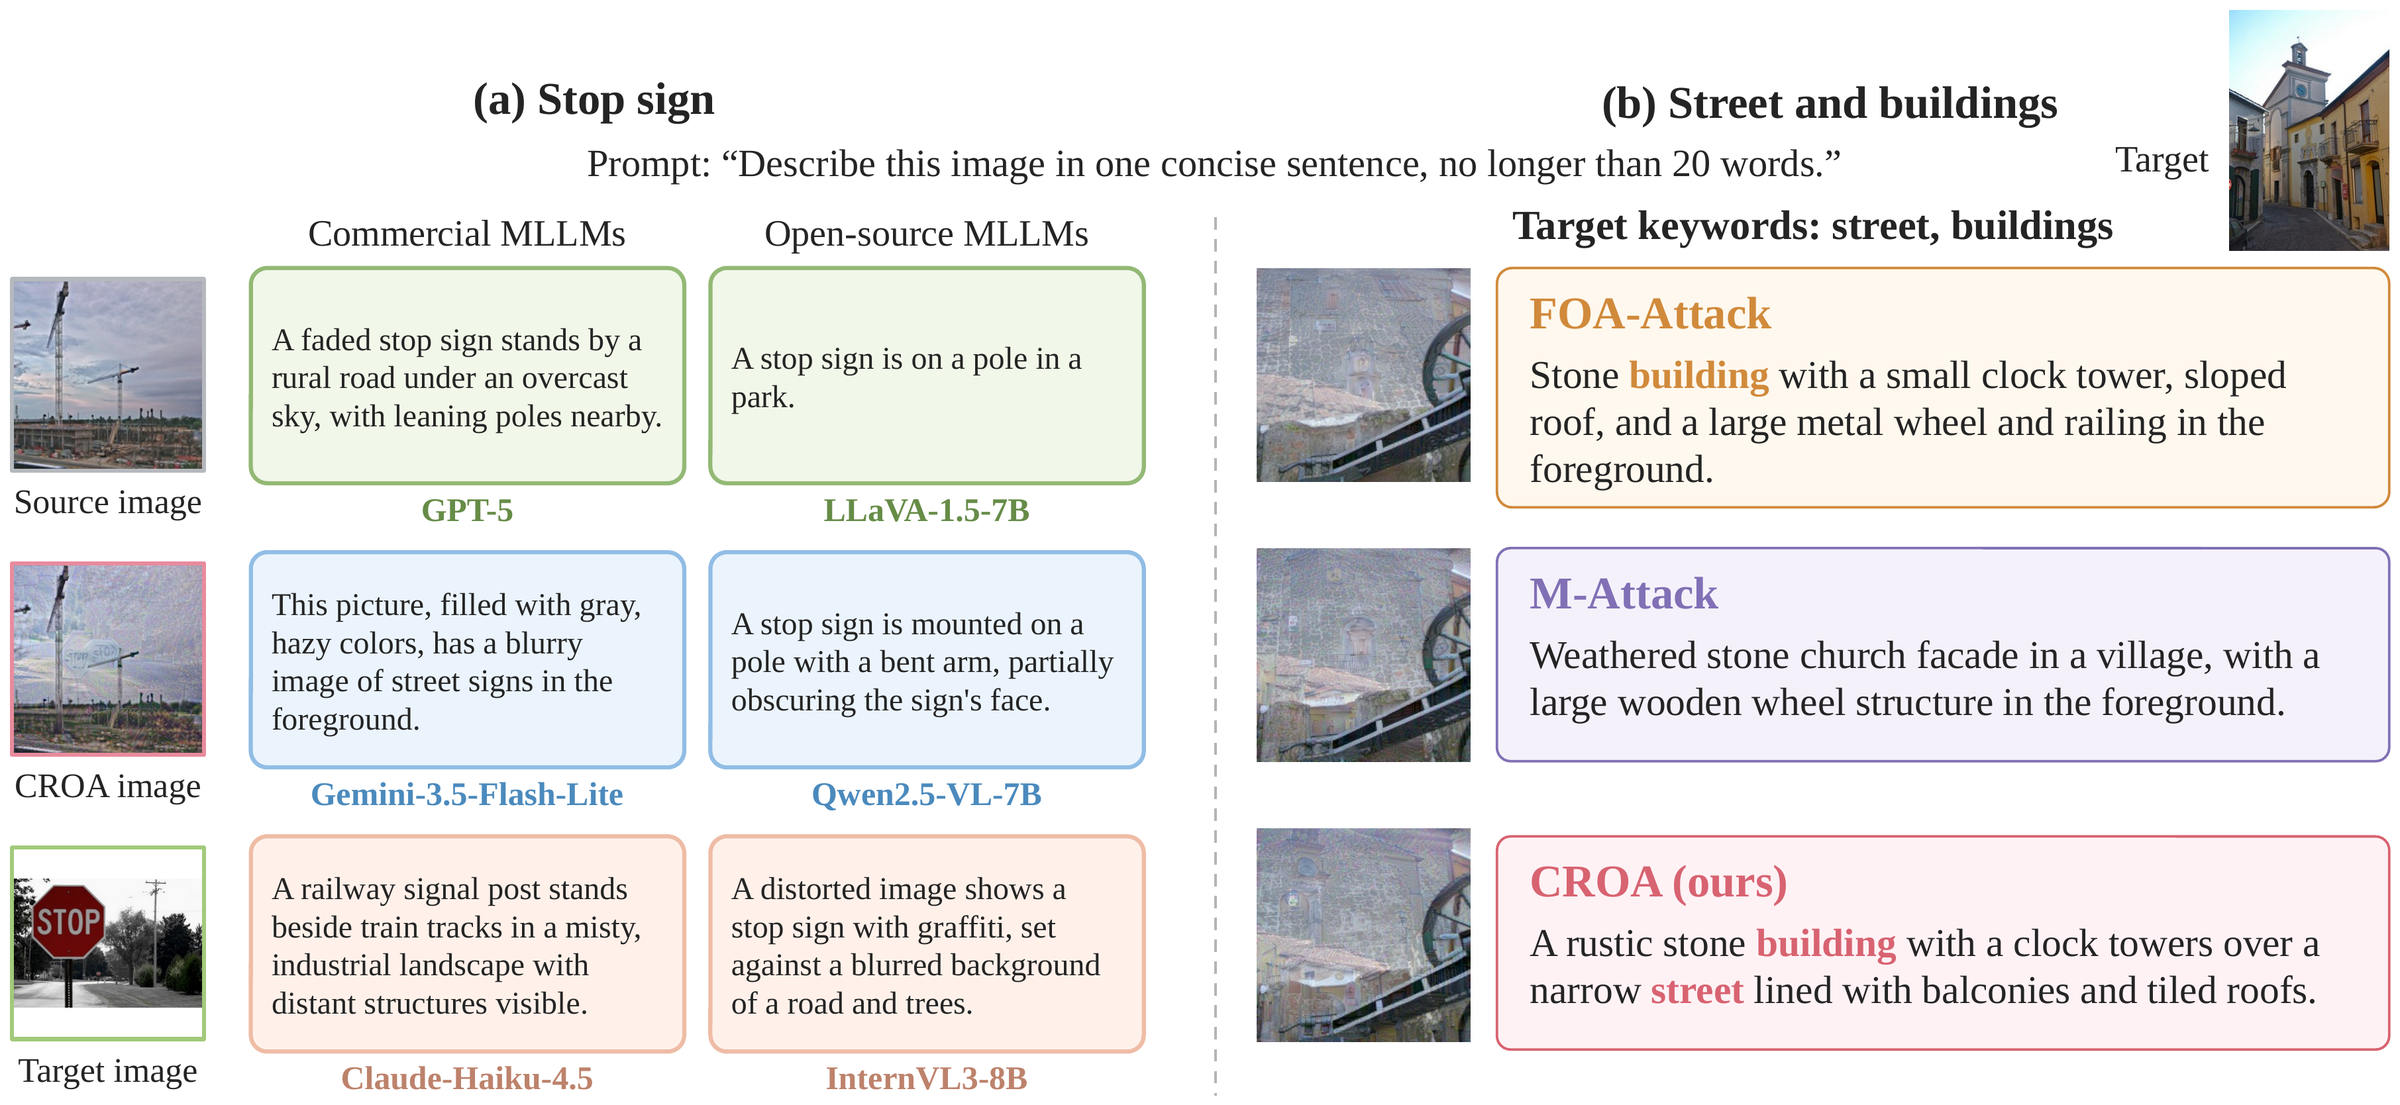
\includegraphics[width=1.02\columnwidth]{assets/ppt_fig3_qualitative.png}}
\vspace{-4pt}
\caption{Selected target-detail examples. Left:
CROA captions from six victims. Right: the CROA caption includes both
``street'' and ``building,'' illustrating keyword coverage beyond the
main object.}
\vspace{-6pt}
\label{fig:qualitative}
\end{figure}
Figure~\ref{fig:qualitative} illustrates qualitative results across diverse MLLMs. On the left, \ours{} steers most victims toward target-aligned descriptions (e.g., a stop sign or signal post) while reflecting architectural variations. On the right, \ours{} induces detailed captions covering fine-grained context such as ``street'' and ``building'', demonstrating effective target-detail semantic coverage.

\section{Conclusion}
We investigated whether self-supervised visual representations complement image--text contrastive features in fine-grained targeted transfer attacks. \ours{} combines global feature alignment and clustered local optimal transport across CLIP and DINOv2 representations, with source repulsion and multi-crop momentum optimization. On 100 source--target pairs, \ours{} achieves mean attack success rates of 51.0\% across three commercial victims and 92.0\% across three open-source victims, the highest among the baselines evaluated under our protocol. Its mean target-keyword recall on the commercial victims is 41.3\%. Component ablations show that DINOv2, local transport, and source repulsion each improve aggregate attack success, although their effects vary across victims. These results support cross-representation alignment for vision-only perturbation generation without target descriptions or an MLLM surrogate.

\clearpage
\balance\begin{thebibliography}{22}
\bibitem{flamingo} J.-B. Alayrac \emph{et al.}, ``Flamingo: A visual language model for few-shot learning,'' in \emph{NeurIPS}, 2022.
\bibitem{blip2} J. Li, D. Li, S. Savarese, and S. Hoi, ``BLIP-2: Bootstrapping language-image pre-training with frozen image encoders and large language models,'' in \emph{ICML}, 2023.
\bibitem{attackvlm} Y. Zhao, T. Pang, C. Du, X. Yang, C. Li, N.-M. Cheung, and M. Lin, ``On evaluating adversarial robustness of large vision-language models,'' in \emph{NeurIPS}, 2023.
\bibitem{mattack} Z. Li \emph{et al.}, ``A frustratingly simple yet highly effective attack baseline: Over 90\% success rate against the strong black-box models of GPT-4.5/4o/o1,'' in \emph{NeurIPS}, 2025.
\bibitem{foa} X. Jia \emph{et al.}, ``Adversarial attacks against closed-source MLLMs via feature optimal alignment,'' in \emph{NeurIPS}, 2025.
\bibitem{ita} X. Cai, D. Liu, R. Guan, and P. Zhou, ``Imperceptible transfer attack on large vision-language models,'' in \emph{ICASSP}, 2025.
\bibitem{gptscore} J. Fu, S.-K. Ng, Z. Jiang, and P. Liu, ``GPTScore: Evaluate as you desire,'' in \emph{NAACL}, 2024.
\bibitem{mifgsm} Y. Dong \emph{et al.}, ``Boosting adversarial attacks with momentum,'' in \emph{CVPR}, 2018.
\bibitem{clip} A. Radford \emph{et al.}, ``Learning transferable visual models from natural language supervision,'' in \emph{ICML}, 2021.
\bibitem{laion} M. Schuhmann \emph{et al.}, ``LAION-5B: An open large-scale dataset for training next generation image-text models,'' in \emph{NeurIPS Datasets and Benchmarks}, 2022.
\bibitem{anyattack} J. Zhang \emph{et al.}, ``AnyAttack: Towards general cross-modal targeted adversarial attacks,'' in \emph{CVPR}, 2025.
\bibitem{sinkhorn} R. Sinkhorn and P. Knopp, ``Concerning nonnegative matrices and doubly stochastic matrices,'' \emph{Pacific J. Math.}, vol. 21, no. 2, pp. 343--348, 1967.
\bibitem{cuturi} M. Cuturi, ``Sinkhorn distances: Lightspeed computation of optimal transport,'' in \emph{NeurIPS}, 2013.
\bibitem{mpcattack} Y. Li \emph{et al.}, ``Multi-paradigm collaborative adversarial attack against multi-modal large language models,'' in \emph{CVPR}, 2026.
\bibitem{dinov2} M. Oquab \emph{et al.}, ``DINOv2: Learning robust visual features without supervision,'' \emph{TMLR}, 2024.
\bibitem{gpt5} OpenAI, ``GPT-5 system card,'' OpenAI Technical Report, 2025.
\bibitem{gemini} Google DeepMind, ``Gemini 3.5 Flash-Lite documentation,'' \emph{Google AI Documentation}, 2026.
\bibitem{claude} Anthropic, ``Claude Haiku 4.5 system card,'' \emph{Anthropic System Card}, 2025.
\bibitem{llava} H. Liu \emph{et al.}, ``Visual instruction tuning,'' in \emph{NeurIPS}, 2023.
\bibitem{qwenvl} S. Bai \emph{et al.}, ``Qwen2.5-VL technical report,'' \emph{arXiv preprint arXiv:2502.13923}, 2025.
\bibitem{internvl} J. Zhu \emph{et al.}, ``InternVL3: Exploring advanced training and test-time recipes for open-source multimodal models,'' \emph{arXiv:2504.10479}, 2025.
\bibitem{gpt4} OpenAI, ``GPT-4o mini: Advancing cost-efficient intelligence,'' OpenAI Tech. Report, 2024.
\end{thebibliography}

\end{document}
